\chapter{Hajautustaulu}

\emph{Hajautustaulu} on tietorakenne,
joka pitää yllä alkioiden joukkoa ja tarjoaa
seuraavat operaatiot:

\begin{itemize}
\item lisää alkio joukkoon
\item tarkasta, onko alkio joukossa
\item poista alkio joukosta
\end{itemize}

Hajautustaulun hienoutena on, että saamme toteutettua
kaikki yllä olevat operaatiot \emph{tehokkaasti},
minkä ansiosta voimme luoda hajautustaulun avulla
tehokkaita algoritmeja.
Mutta ennen kuin alamme käyttää hajautustaulua,
on paikallaan ottaa selvää, miten se toimii.

\section{Hajautustaulun toiminta}

\begin{figure}
\center
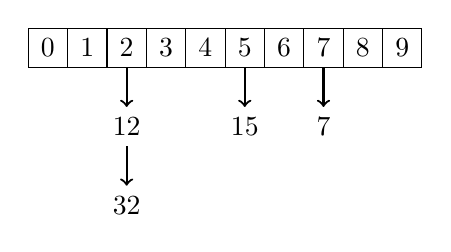
\begin{tikzpicture}[scale=0.5]
\draw (0,0) grid (10,1);
\foreach \x in {0,1,...,9} \node at (0.5+\x,0.5) {\x};
\draw[->,thick] (2.5,0) -- (2.5,-1);
\draw[->,thick] (5.5,0) -- (5.5,-1);
\draw[->,thick] (7.5,0) -- (7.5,-1);
\draw[->,thick] (2.5,-2) -- (2.5,-3);
\node at (2.5,-1.5) {$12$};
\node at (5.5,-1.5) {$15$};
\node at (7.5,-1.5) {$7$};
\node at (2.5,-3.5) {$32$};
\end{tikzpicture}
\caption{Hajautustaulu, joka vastaa joukkoa $\{7,12,15,32\}$.
Hajautusfunktiona on $f(x)=x \bmod 10$.}
\label{fig:hajtau}
\end{figure}

Toteutamme hajautustaulun taulukkona,
jonka jokaisessa kohdassa on lista joukkoon kuuluvia alkioita.
Jotta voimme käyttää hajautustaulua,
tarvitsemme \emph{hajautusfunktion} $f$,
joka antaa \emph{hajautusarvon}
$f(x)$ mille tahansa joukon alkiolle $x$.
Hajautusarvo on kokonaisluku väliltä
$0,1,\dots,N-1$, missä $N$ on hajautustaulun koko.
Tallennamme hajautustaulun kohdassa $k$ olevaan listaan
kaikki ne joukon alkiot, joiden hajautusarvo on $k$.

Kuvassa \ref{fig:hajtau} on esimerkkinä hajautustaulu,
jonka kokona on $N=10$.
Olemme tallentaneet hajautustauluun joukon $\{7,12,15,32\}$
käyttäen hajautusfunktiota $f(x)=x \bmod 10$.
Tämä tarkoittaa, että alkion $x$ hajautusarvo on sen jakojäännös $10$:llä
eli luvun viimeinen numero.
Esimerkiksi alkiot $12$ ja $32$ ovat kohdassa $2$,
koska niissä viimeinen numero on $2$,
ja alkiot $15$ ja $7$ ovat vastaavasti kohdissa $5$ ja $7$.
Kaikki muut hajautustaulun listat ovat tällä hetkellä tyhjiä.

Kun haluamme tarkastaa, onko joukossa alkiota $x$,
laskemme ensin sen hajautusarvon $f(x)$.
Tämän jälkeen käymme läpi kaikki kohdan $f(x)$
listassa olevat alkiot ja tarkastamme,
onko jokin niistä alkio $x$.
Vastaavasti kun haluamme lisätä alkion $x$ joukkoon
tai poistaa alkion $x$ joukosta,
teemme muutoksen kohdassa $f(x)$ olevaan listaan.
Jokaisen operaation aikavaativuus on $O(m)$,
missä $m$ on listan alkioiden määrä.
Hajautustaulu toimii siis tehokkaasti, jos jokainen
siinä oleva lista on lyhyt.

\subsection{Hajautusfunktio}

Hajautusfunktio $f(x)$ määrittää, mihin kohtaan hajautustaulua
alkio $x$ sijoitetaan.
Sen täytyy antaa jokaiselle mahdolliselle alkiolle
hajautusarvo eli kokonaisluku väliltä $0,1,\dots,N-1$,
missä $N$ on hajautustaulun koko.
Muilta osin meillä on periaatteessa vapaat kädet
hajautusfunktion suunnitteluun.
Mutta millainen olisi hyvä hajautusfunktio?

\begin{figure}
\center
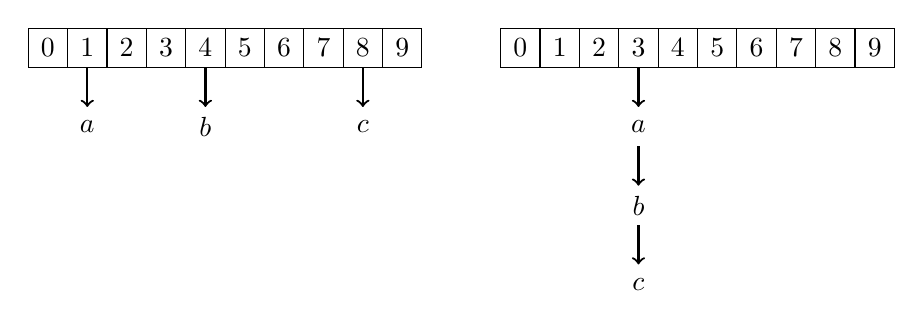
\begin{tikzpicture}[scale=0.5]
\begin{scope}
\draw (0,0) grid (10,1);
\foreach \x in {0,1,...,9} \node at (0.5+\x,0.5) {\x};
\draw[->,thick] (1.5,0) -- (1.5,-1);
\draw[->,thick] (4.5,0) -- (4.5,-1);
\draw[->,thick] (8.5,0) -- (8.5,-1);
\node at (1.5,-1.5) {$a$};
\node at (4.5,-1.5) {$b$};
\node at (8.5,-1.5) {$c$};
\end{scope}
\begin{scope}[xshift=12cm]
\draw (0,0) grid (10,1);
\foreach \x in {0,1,...,9} \node at (0.5+\x,0.5) {\x};
\draw[->,thick] (3.5,0) -- (3.5,-1);
\draw[->,thick] (3.5,-4) -- (3.5,-5);
\draw[->,thick] (3.5,-2) -- (3.5,-3);
\node at (3.5,-1.5) {$a$};
\node at (3.5,-3.5) {$b$};
\node at (3.5,-5.5) {$c$};
\end{scope}
\end{tikzpicture}
\caption{Kaksi hajautustaulua joukolle $\{a,b,c\}$.
Vasen tilanne on paras mahdollinen, oikea tilanne taas
huonoin mahdollinen.}
\label{fig:hajjak}
\end{figure}

Haluamme, että hajautusfunktio jakaa alkioita \emph{tasaisesti}
hajautustaulun eri puolille.
Jos onnistumme tässä, kaikki listat ovat lyhyitä ja
hajautustaulun operaatiot ovat tehokkaita.
Kuva \ref{fig:hajjak} näyttää kaksi hajautustaulua, jotka vastaavat
joukkoa $\{a,b,c\}$ kahdella eri hajautusfunktiolla.
Vasemmassa taulussa hajautus on onnistunut täydellisesti
ja jokainen alkio on omassa listassaan.
Oikeassa taulussa taas kaikki alkiot ovat joutuneet samaan
listaan eikä hajautuksesta ole mitään hyötyä.
Tavoitteemme on saada aikaan hajautusfunktio,
jonka toiminta on lähempänä vasenta tilannetta.

Jos hajautettavat alkiot ovat kokonaislukuja,
suoraviivainen hajautusfunktio on $f(x)=x \bmod N$,
mikä tarkoittaa, että otamme jakojäännöksen hajautustaulun koolla $N$.
Tämä on hyvin toimiva hajautusfunktio,
kunhan aineistossa esiintyy tasaisesti eri jakojäännöksiä.
Entä jos alkiot ovat jotain muuta tyyppiä kuin kokonaislukuja?
Tällöin meidän riittää päättää ensin jokin järkevä tapa,
kuinka muutamme alkion kokonaisluvuksi,
minkä jälkeen otamme jakojäännöksen $N$:llä.

Tarkastellaan tilannetta, jossa haluamme hajauttaa merkkijonoja
eli mei\-dän täytyy löytää keino muuttaa merkkijono kokonaisluvuksi.
Oletamme, että merkkijonossa on $k$ merkkiä,
joiden merkkikoodit ovat $c_0,c_1,\dots,c_{k-1}$.
Esimerkiksi jos merkkijono on \texttt{apina},
merkkikoodit\footnote{Käytämme tässä merkkien ASCII-koodeja.
Esimerkiksi Javassa char-merkin \texttt{c} koodin saa
selville kirjoittamalla \texttt{(int)c}, eli esimerkiksi
\texttt{(int)'a'} on 97.} ovat $c_0=97$, $c_1=112$, $c_2=105$,
$c_3=110$ ja $c_4=97$.
Yksi tapa muuttaa merkkijono kokonaisluvuksi
on laskea merkkikoodien summa
\[ c_0 + c_1 + \dots + c_{k-1},\]
jolloin merkkijonon \texttt{apina} hajautusarvo on
\[97+112+105+110+97=521.\]

Tämä on sinänsä järkevä tapa, mutta siinä on yksi ongelma:
kaksi merkkijonoa saavat aina saman hajautusarvon,
jos niissä on samat merkit eri järjestyksessä.
Pystymme parantamaan hajautusarvon laskentaa lisäämällä
summaan \emph{kertoimet} käyttäen kaavaa
\[ A^{k-1} c_0 + A^{k-2} c_1 + \dots + A^0 c_{k-1},\]
missä $A$ on vakio.
Esimerkiksi jos $A=7$, saamme merkkijonon \texttt{apina} hajautusarvoksi
\[7^4 \cdot 97+7^3 \cdot 112+7^2 \cdot 105+7^1 \cdot 110+7^0 \cdot 97=61235.\]
Tämä menetelmä, jota kutsutaan nimellä \emph{polynominen hajautus},
on käytän\-nössä hyvä merkkijonon hajautustapa,
joka on käytössä esimerkiksi Javan standardikirjastossa.

\subsection{Hajautuksen tehokkuus}

Hajautustaulun operaatiot vievät aikaa $O(m)$,
jossa $m$ on hajautustaulussa olevan listan pituus.
Mutta kuinka suuri $m$ on? Tämä riippuu siitä,
mikä on alkioiden määrä $n$, hajautustaulun koko $N$
sekä hajautusfunktio $f$.

Jos kaikki sujuu hyvin ja hajautusfunktio jakaa alkioita
tasaisesti hajautustaulun eri puolille,
jokaisessa listassa on noin $n/N$ alkiota.
Niinpä jos valitsemme hajautustaulun koon niin,
että $N$ on samaa luokkaa kuin $n$,
operaatiot toimivat tehokkaasti ajassa $O(1)$.
Kuitenkin on mahdollista että hajautus epäonnistuu
ja alkiot jakautuvat hajautustauluun epätasaisesti.
Pahimmassa tapauksessa kaikki alkiot saavat saman
hajautusarvon ja ne kaikki tallennetaan samaan listaan,
jolloin operaatiot vievät aikaa $O(n)$.

Voimme helposti vaikuttaa hajautustaulun kokoon $N$,
mutta hajautusfunktion suunnittelu on epämääräisempi ala.
Miten voimme tietää, että valitsemamme hajautusfunktio
toimii hyvin?
Itse asiassa emme voi olla koskaan varmoja tästä.
Vaikka meillä olisi erittäin hyvä hajautusfunktio,
\emph{ilkeä vastustaja} voi kuitenkin antaa
meille joukon alkioita, jotka kaikki saavat saman hajautusarvon.
Tämä riski on aina hajautuksessa, koska mahdollisten
hajautusarvojen määrä on paljon pienempi kuin mahdollisten alkioiden määrä.
Tämän vuoksi emme voi mitenkään suunnitella hajautusfunktiota niin,
että se jakaisi alkiot \emph{varmasti} tasaisesti hajautustauluun.

Kaikeksi onneksi hajautus toimii yleensä aina \emph{käytännössä}
hyvin ja voimme ajatella, että hajautustaulun operaatiot ovat
$O(1)$-aikaisia, kunhan hajautustaulun koko on riittävän suuri ja
hajautusfunktio on toteutettu järke\-västi.
Vaikka on mahdollista, että hajautus epäonnistuu,
tämän riski on niin pieni, että meidän ei tarvitse murehtia
siitä käytännössä.

\subsection{Joukosta hakemistoksi}

Voimme luoda hajautustaulun avulla myös tietorakenteen
\emph{hakemisto}, joka sisältää joukon avain-arvo-pareja.
Voimme ajatella hakemistoa taulukon yleistyksenä:
taulukossa avaimet ovat kokonaisluvut $0,1,\dots,n-1$,
mutta hakemistossa ne voivat olla mitä tahansa.
Avaimen hajautusarvo ratkaisee, mihin hajautustaulun
listaan pari sijoitetaan.

Kuvassa \ref{fig:hajhak} on esimerkkinä hajautustauluun
tallennettu hakemisto, joka vastaa seuraavaa ''taulukkoa'':

\begin{code}
taulu["abc"] = 5
taulu["xyz"] = 1
taulu["aaa"] = 8
\end{code}

Tässä tapauksessa hakemiston avaimet ovat merkkijonoja
ja avaimet ovat kokonaislukuja.
Hajautustaulun ansiosta voimme käsitellä hakemistoa
taulukon tavoin niin, että operaatiot vievät aikaa $O(1)$.

\begin{figure}
\center
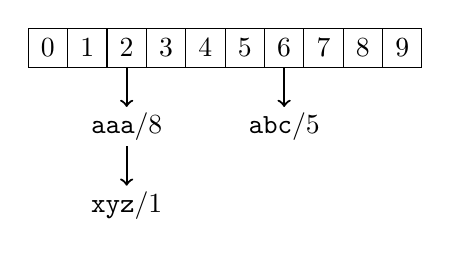
\begin{tikzpicture}[scale=0.5]
\draw (0,0) grid (10,1);
\foreach \x in {0,1,...,9} \node at (0.5+\x,0.5) {\x};
\draw[->,thick] (2.5,0) -- (2.5,-1);
\draw[->,thick] (6.5,0) -- (6.5,-1);
\draw[->,thick] (2.5,-2) -- (2.5,-3);
\node at (2.5,-1.5) {$\texttt{aaa}/8$};
\node at (2.5,-3.5) {$\texttt{xyz}/1$};
\node at (6.5,-1.5) {$\texttt{abc}/5$};
\end{tikzpicture}
\caption{Hakemiston tallentaminen hajautustauluun.}
\label{fig:hajhak}
\end{figure}

\section{Javan toteutukset}

Javassa on kaksi hajautustaulua käyttävää tietorakennetta:
\texttt{HashSet} pitää yllä alkioiden joukkoa
ja \texttt{HashMap} toteuttaa
hakemiston, jossa on avain-arvo-pareja.
Seuraavaksi tutustumme tarkemmin näihin rakenteisiin.

\subsection{\texttt{HashSet}-rakenne}

\texttt{HashSet} on alkioiden joukko,
johon voi lisätä alkion metodilla \texttt{add}
ja josta voi poistaa alkion metodilla \texttt{remove}.
Esimerkiksi seuraava koodi luo joukon, jossa voi olla
kokonaislukuja, ja lisää siihen luvut 3, 5 ja 8.
Tämän jälkeen koodi poistaa luvun 5 joukosta.

\begin{code}
HashSet<Integer> joukko = new HashSet<>();
joukko.add(3);
joukko.add(5);
joukko.add(8);
System.out.println(joukko); // [3, 5, 8]
joukko.remove(5);
System.out.println(joukko); // [3, 8]
\end{code}

Metodi \texttt{contains} kertoo, esiintyykö tietty alkio $x$ joukossa:

\begin{code}
if (joukko.contains(x)) {
    System.out.println("alkio on joukossa");
} else {
    System.out.println("alkiota ei ole joukossa");
}
\end{code}

Huomaa, että jokainen alkio voi esiintyä vain kerran joukossa.
Esimerkiksi vaikka seuraava koodi lisää luvun 5 kolmesti
joukkoon, se menee sinne vain ensimmäisellä kerralla ja
muut lisäykset jätetään huomiotta.

\begin{code}
HashSet<Integer> joukko = new HashSet<>();
joukko.add(5);
joukko.add(5);
joukko.add(5);
System.out.println(joukko); // [5]
\end{code}

Koska \texttt{HashSet} on toteutettu hajautustaulun avulla,
sen operaatiot toimivat ajassa $O(1)$.

\subsection{\texttt{HashMap}-rakenne}

\texttt{HashMap} luo hakemiston,
jossa on avain-arvo-pareja.
Hakemiston määrit\-telyssä tulee antaa
avaimen ja arvon tyyppi.
Metodi \texttt{put} lisää uuden avain-arvo-parin,
ja metodi \texttt{get} hakee arvon avaimen perusteella.

Esimerkiksi seuraava koodi luo sanakirjan, jossa sekä
avaimet että arvot ovat merkkijonoja.
Syötämme sanakirjaan merkkijonopareja, jotka kertovat
sanan käännöksen suomesta englanniksi.

\begin{code}
HashMap<String,String> sanakirja = new HashMap<>();

sanakirja.put("apina","monkey");
sanakirja.put("banaani","banana");
sanakirja.put("cembalo","harpsichord");

System.out.println(sanakirja.get("banaani")); // banana
\end{code}

Hyödyllinen on myös metodi \texttt{containsKey},
jonka avulla voi tarkastaa, onko tietylle avaimelle
tallennettu arvoa:

\begin{code}
if (sanakirja.containsKey(sana)) {
    System.out.println("Käännös: " + sanakirja.get(sana));
} else {
    System.out.println("Sana puuttuu sanakirjasta!");
}
\end{code}

Koska \texttt{HashMap} on toteutettu hajautustaulun avulla,
sen operaatiot toimivat ajassa $O(1)$.

\subsection{Omat luokat}

Javan luokissa on metodi \texttt{hashCode},
jonka avulla olio kertoo pyydettäessä hajautusarvonsa.
Voimme esimerkiksi selvittää merkkijonon \texttt{apina}
hajautusarvon seuraavasti:

\begin{code}
System.out.println("apina".hashCode());
\end{code}

Tämä koodi tulostaa luvun 93022541,
joka on siis merkkijonon \texttt{apina} hajautusarvo Javassa.
On tunnettua, että Java käyttää merkkijonon hajautusarvon laskemiseen
polynomista hajautusta vakiolla $A=31$,
joten voimme laskea Javan hajautusarvon myös itse kaavalla
\[31^4 \cdot 97+31^3 \cdot 112+31^2 \cdot 105+31^1 \cdot 110+31^0 \cdot 97=93022541.\]

Jos haluamme käyttää omia oliota hajautustauluissa,
meidän täytyy toteuttaa luokkaan kaksi metodia:
\texttt{hashCode}, joka antaa olion hajautusarvon,
sekä \texttt{equals},
joka ilmaisee, ovatko kaksi oliota samat.
Metodi \texttt{hashCode} riittää toteuttaa niin,
että se palauttaa jonkin kokonaisluvun.
Metodi \texttt{equals} on tarpeen,
jotta Java pystyy varmistamaan, ovatko saman hajautusarvon
antavat oliot todella samat.

\section{Joukot algoritmiikassa}

Hajautustaulun ansiosta voimme käyttää algoritmeissamme
joukkoja ja hakemistoja, joiden operaatiot toimivat tehokkaasti.
Voimme alkajaisiksi ratkaista mukavammin ajassa $O(n)$ sellaisia ongelmia,
jotka olemme ratkoneet aiemmin luvussa 3.5
järjestämisen avulla ajassa $O(n \log n)$

Aloitamme ongelmasta, jossa haluamme selvittää,
montako eri alkiota taulukko sisältää.
Nyt kun käytössämme on hajautustaulu, voimme vain lisätä
kaikki alkiot joukkoon ja hakea lopuksi joukon koon.
Näin saamme aikaan seuraavan algoritmin:

\begin{code}
alkiot = []
for i = 0 to n-1
    alkiot.add(taulu[i])
print(alkiot.size())
\end{code}

Entä jos haluamme selvittää, mikä on taulukon yleisin alkio?
Hajautustaulun avulla voimme lähestyä ongelmaa
luomalla hakemiston,
jonka avaimet ovat taulukon alkioita ja arvot niiden
esiintymiskertoja.
Nyt voimme vain käydä läpi taulukon sisällön ja
pitää kirjaa, montako kertaa mikäkin alkio esiintyy taulukossa:

\begin{code}
kerrat = []
suurin = 1
yleisin = taulu[0]
for i = 0 to n-1
    kerrat[taulu[i]]++
    if kerrat[taulu[i]] > suurin
        suurin = kerrat[taulu[i]]
        yleisin = taulu[i]
print(yleisin)
\end{code}

Kuten nämä esimerkit osoittavat, hajautustaulu
helpottaa algoritmien luomista,
koska meidän ei tarvitse kikkailla järjestämisen kanssa.
Mutta nyt\-hän olemme vain ratkoneet uudestaan tehtäviä,
jotka hoituvat mainiosti myös järjestämisen avulla.
Antaisiko hajautustaulu meille aitoja uusia mahdollisuuksia
algoritmien suunnittelussa?

Hajautustaulun todellinen merkitys on siinä, että voimme sekä
\emph{lisätä} että \emph{poistaa} alkioita tehokkaasti milloin vain haluamme
algoritmin aikana.
Jos algoritmi vain lisää alkioita,
kuten olemme tehneet tähän mennessä,
voimme yleensä tavalla tai toisella keksiä korvaavan algoritmin,
joka käyttää hajautustaulun sijasta järjestämistä.
Mutta jos algoritmissa esiintyy sekä lisäyksiä että poistoja,
emme ehkä löydä enää vaihtoehtoja hajautustaululle.